
% Default to the notebook output style

    


% Inherit from the specified cell style.




    
\documentclass[11pt]{article}

    
    
    \usepackage[T1]{fontenc}
    % Nicer default font (+ math font) than Computer Modern for most use cases
    \usepackage{mathpazo}

    % Basic figure setup, for now with no caption control since it's done
    % automatically by Pandoc (which extracts ![](path) syntax from Markdown).
    \usepackage{graphicx}
    % We will generate all images so they have a width \maxwidth. This means
    % that they will get their normal width if they fit onto the page, but
    % are scaled down if they would overflow the margins.
    \makeatletter
    \def\maxwidth{\ifdim\Gin@nat@width>\linewidth\linewidth
    \else\Gin@nat@width\fi}
    \makeatother
    \let\Oldincludegraphics\includegraphics
    % Set max figure width to be 80% of text width, for now hardcoded.
    \renewcommand{\includegraphics}[1]{\Oldincludegraphics[width=.8\maxwidth]{#1}}
    % Ensure that by default, figures have no caption (until we provide a
    % proper Figure object with a Caption API and a way to capture that
    % in the conversion process - todo).
    \usepackage{caption}
    \DeclareCaptionLabelFormat{nolabel}{}
    \captionsetup{labelformat=nolabel}

    \usepackage{adjustbox} % Used to constrain images to a maximum size 
    \usepackage{xcolor} % Allow colors to be defined
    \usepackage{enumerate} % Needed for markdown enumerations to work
    \usepackage{geometry} % Used to adjust the document margins
    \usepackage{amsmath} % Equations
    \usepackage{amssymb} % Equations
    \usepackage{textcomp} % defines textquotesingle
    % Hack from http://tex.stackexchange.com/a/47451/13684:
    \AtBeginDocument{%
        \def\PYZsq{\textquotesingle}% Upright quotes in Pygmentized code
    }
    \usepackage{upquote} % Upright quotes for verbatim code
    \usepackage{eurosym} % defines \euro
    \usepackage[mathletters]{ucs} % Extended unicode (utf-8) support
    \usepackage[utf8x]{inputenc} % Allow utf-8 characters in the tex document
    \usepackage{fancyvrb} % verbatim replacement that allows latex
    \usepackage{grffile} % extends the file name processing of package graphics 
                         % to support a larger range 
    % The hyperref package gives us a pdf with properly built
    % internal navigation ('pdf bookmarks' for the table of contents,
    % internal cross-reference links, web links for URLs, etc.)
    \usepackage{hyperref}
    \usepackage{longtable} % longtable support required by pandoc >1.10
    \usepackage{booktabs}  % table support for pandoc > 1.12.2
    \usepackage[inline]{enumitem} % IRkernel/repr support (it uses the enumerate* environment)
    \usepackage[normalem]{ulem} % ulem is needed to support strikethroughs (\sout)
                                % normalem makes italics be italics, not underlines
    

    
    
    % Colors for the hyperref package
    \definecolor{urlcolor}{rgb}{0,.145,.698}
    \definecolor{linkcolor}{rgb}{.71,0.21,0.01}
    \definecolor{citecolor}{rgb}{.12,.54,.11}

    % ANSI colors
    \definecolor{ansi-black}{HTML}{3E424D}
    \definecolor{ansi-black-intense}{HTML}{282C36}
    \definecolor{ansi-red}{HTML}{E75C58}
    \definecolor{ansi-red-intense}{HTML}{B22B31}
    \definecolor{ansi-green}{HTML}{00A250}
    \definecolor{ansi-green-intense}{HTML}{007427}
    \definecolor{ansi-yellow}{HTML}{DDB62B}
    \definecolor{ansi-yellow-intense}{HTML}{B27D12}
    \definecolor{ansi-blue}{HTML}{208FFB}
    \definecolor{ansi-blue-intense}{HTML}{0065CA}
    \definecolor{ansi-magenta}{HTML}{D160C4}
    \definecolor{ansi-magenta-intense}{HTML}{A03196}
    \definecolor{ansi-cyan}{HTML}{60C6C8}
    \definecolor{ansi-cyan-intense}{HTML}{258F8F}
    \definecolor{ansi-white}{HTML}{C5C1B4}
    \definecolor{ansi-white-intense}{HTML}{A1A6B2}

    % commands and environments needed by pandoc snippets
    % extracted from the output of `pandoc -s`
    \providecommand{\tightlist}{%
      \setlength{\itemsep}{0pt}\setlength{\parskip}{0pt}}
    \DefineVerbatimEnvironment{Highlighting}{Verbatim}{commandchars=\\\{\}}
    % Add ',fontsize=\small' for more characters per line
    \newenvironment{Shaded}{}{}
    \newcommand{\KeywordTok}[1]{\textcolor[rgb]{0.00,0.44,0.13}{\textbf{{#1}}}}
    \newcommand{\DataTypeTok}[1]{\textcolor[rgb]{0.56,0.13,0.00}{{#1}}}
    \newcommand{\DecValTok}[1]{\textcolor[rgb]{0.25,0.63,0.44}{{#1}}}
    \newcommand{\BaseNTok}[1]{\textcolor[rgb]{0.25,0.63,0.44}{{#1}}}
    \newcommand{\FloatTok}[1]{\textcolor[rgb]{0.25,0.63,0.44}{{#1}}}
    \newcommand{\CharTok}[1]{\textcolor[rgb]{0.25,0.44,0.63}{{#1}}}
    \newcommand{\StringTok}[1]{\textcolor[rgb]{0.25,0.44,0.63}{{#1}}}
    \newcommand{\CommentTok}[1]{\textcolor[rgb]{0.38,0.63,0.69}{\textit{{#1}}}}
    \newcommand{\OtherTok}[1]{\textcolor[rgb]{0.00,0.44,0.13}{{#1}}}
    \newcommand{\AlertTok}[1]{\textcolor[rgb]{1.00,0.00,0.00}{\textbf{{#1}}}}
    \newcommand{\FunctionTok}[1]{\textcolor[rgb]{0.02,0.16,0.49}{{#1}}}
    \newcommand{\RegionMarkerTok}[1]{{#1}}
    \newcommand{\ErrorTok}[1]{\textcolor[rgb]{1.00,0.00,0.00}{\textbf{{#1}}}}
    \newcommand{\NormalTok}[1]{{#1}}
    
    % Additional commands for more recent versions of Pandoc
    \newcommand{\ConstantTok}[1]{\textcolor[rgb]{0.53,0.00,0.00}{{#1}}}
    \newcommand{\SpecialCharTok}[1]{\textcolor[rgb]{0.25,0.44,0.63}{{#1}}}
    \newcommand{\VerbatimStringTok}[1]{\textcolor[rgb]{0.25,0.44,0.63}{{#1}}}
    \newcommand{\SpecialStringTok}[1]{\textcolor[rgb]{0.73,0.40,0.53}{{#1}}}
    \newcommand{\ImportTok}[1]{{#1}}
    \newcommand{\DocumentationTok}[1]{\textcolor[rgb]{0.73,0.13,0.13}{\textit{{#1}}}}
    \newcommand{\AnnotationTok}[1]{\textcolor[rgb]{0.38,0.63,0.69}{\textbf{\textit{{#1}}}}}
    \newcommand{\CommentVarTok}[1]{\textcolor[rgb]{0.38,0.63,0.69}{\textbf{\textit{{#1}}}}}
    \newcommand{\VariableTok}[1]{\textcolor[rgb]{0.10,0.09,0.49}{{#1}}}
    \newcommand{\ControlFlowTok}[1]{\textcolor[rgb]{0.00,0.44,0.13}{\textbf{{#1}}}}
    \newcommand{\OperatorTok}[1]{\textcolor[rgb]{0.40,0.40,0.40}{{#1}}}
    \newcommand{\BuiltInTok}[1]{{#1}}
    \newcommand{\ExtensionTok}[1]{{#1}}
    \newcommand{\PreprocessorTok}[1]{\textcolor[rgb]{0.74,0.48,0.00}{{#1}}}
    \newcommand{\AttributeTok}[1]{\textcolor[rgb]{0.49,0.56,0.16}{{#1}}}
    \newcommand{\InformationTok}[1]{\textcolor[rgb]{0.38,0.63,0.69}{\textbf{\textit{{#1}}}}}
    \newcommand{\WarningTok}[1]{\textcolor[rgb]{0.38,0.63,0.69}{\textbf{\textit{{#1}}}}}
    
    
    % Define a nice break command that doesn't care if a line doesn't already
    % exist.
    \def\br{\hspace*{\fill} \\* }
    % Math Jax compatability definitions
    \def\gt{>}
    \def\lt{<}
    % Document parameters
    \title{Introduction to Recommender Systems in Python}
    
    
    

    % Pygments definitions
    
\makeatletter
\def\PY@reset{\let\PY@it=\relax \let\PY@bf=\relax%
    \let\PY@ul=\relax \let\PY@tc=\relax%
    \let\PY@bc=\relax \let\PY@ff=\relax}
\def\PY@tok#1{\csname PY@tok@#1\endcsname}
\def\PY@toks#1+{\ifx\relax#1\empty\else%
    \PY@tok{#1}\expandafter\PY@toks\fi}
\def\PY@do#1{\PY@bc{\PY@tc{\PY@ul{%
    \PY@it{\PY@bf{\PY@ff{#1}}}}}}}
\def\PY#1#2{\PY@reset\PY@toks#1+\relax+\PY@do{#2}}

\expandafter\def\csname PY@tok@gd\endcsname{\def\PY@tc##1{\textcolor[rgb]{0.63,0.00,0.00}{##1}}}
\expandafter\def\csname PY@tok@gu\endcsname{\let\PY@bf=\textbf\def\PY@tc##1{\textcolor[rgb]{0.50,0.00,0.50}{##1}}}
\expandafter\def\csname PY@tok@gt\endcsname{\def\PY@tc##1{\textcolor[rgb]{0.00,0.27,0.87}{##1}}}
\expandafter\def\csname PY@tok@gs\endcsname{\let\PY@bf=\textbf}
\expandafter\def\csname PY@tok@gr\endcsname{\def\PY@tc##1{\textcolor[rgb]{1.00,0.00,0.00}{##1}}}
\expandafter\def\csname PY@tok@cm\endcsname{\let\PY@it=\textit\def\PY@tc##1{\textcolor[rgb]{0.25,0.50,0.50}{##1}}}
\expandafter\def\csname PY@tok@vg\endcsname{\def\PY@tc##1{\textcolor[rgb]{0.10,0.09,0.49}{##1}}}
\expandafter\def\csname PY@tok@vi\endcsname{\def\PY@tc##1{\textcolor[rgb]{0.10,0.09,0.49}{##1}}}
\expandafter\def\csname PY@tok@vm\endcsname{\def\PY@tc##1{\textcolor[rgb]{0.10,0.09,0.49}{##1}}}
\expandafter\def\csname PY@tok@mh\endcsname{\def\PY@tc##1{\textcolor[rgb]{0.40,0.40,0.40}{##1}}}
\expandafter\def\csname PY@tok@cs\endcsname{\let\PY@it=\textit\def\PY@tc##1{\textcolor[rgb]{0.25,0.50,0.50}{##1}}}
\expandafter\def\csname PY@tok@ge\endcsname{\let\PY@it=\textit}
\expandafter\def\csname PY@tok@vc\endcsname{\def\PY@tc##1{\textcolor[rgb]{0.10,0.09,0.49}{##1}}}
\expandafter\def\csname PY@tok@il\endcsname{\def\PY@tc##1{\textcolor[rgb]{0.40,0.40,0.40}{##1}}}
\expandafter\def\csname PY@tok@go\endcsname{\def\PY@tc##1{\textcolor[rgb]{0.53,0.53,0.53}{##1}}}
\expandafter\def\csname PY@tok@cp\endcsname{\def\PY@tc##1{\textcolor[rgb]{0.74,0.48,0.00}{##1}}}
\expandafter\def\csname PY@tok@gi\endcsname{\def\PY@tc##1{\textcolor[rgb]{0.00,0.63,0.00}{##1}}}
\expandafter\def\csname PY@tok@gh\endcsname{\let\PY@bf=\textbf\def\PY@tc##1{\textcolor[rgb]{0.00,0.00,0.50}{##1}}}
\expandafter\def\csname PY@tok@ni\endcsname{\let\PY@bf=\textbf\def\PY@tc##1{\textcolor[rgb]{0.60,0.60,0.60}{##1}}}
\expandafter\def\csname PY@tok@nl\endcsname{\def\PY@tc##1{\textcolor[rgb]{0.63,0.63,0.00}{##1}}}
\expandafter\def\csname PY@tok@nn\endcsname{\let\PY@bf=\textbf\def\PY@tc##1{\textcolor[rgb]{0.00,0.00,1.00}{##1}}}
\expandafter\def\csname PY@tok@no\endcsname{\def\PY@tc##1{\textcolor[rgb]{0.53,0.00,0.00}{##1}}}
\expandafter\def\csname PY@tok@na\endcsname{\def\PY@tc##1{\textcolor[rgb]{0.49,0.56,0.16}{##1}}}
\expandafter\def\csname PY@tok@nb\endcsname{\def\PY@tc##1{\textcolor[rgb]{0.00,0.50,0.00}{##1}}}
\expandafter\def\csname PY@tok@nc\endcsname{\let\PY@bf=\textbf\def\PY@tc##1{\textcolor[rgb]{0.00,0.00,1.00}{##1}}}
\expandafter\def\csname PY@tok@nd\endcsname{\def\PY@tc##1{\textcolor[rgb]{0.67,0.13,1.00}{##1}}}
\expandafter\def\csname PY@tok@ne\endcsname{\let\PY@bf=\textbf\def\PY@tc##1{\textcolor[rgb]{0.82,0.25,0.23}{##1}}}
\expandafter\def\csname PY@tok@nf\endcsname{\def\PY@tc##1{\textcolor[rgb]{0.00,0.00,1.00}{##1}}}
\expandafter\def\csname PY@tok@si\endcsname{\let\PY@bf=\textbf\def\PY@tc##1{\textcolor[rgb]{0.73,0.40,0.53}{##1}}}
\expandafter\def\csname PY@tok@s2\endcsname{\def\PY@tc##1{\textcolor[rgb]{0.73,0.13,0.13}{##1}}}
\expandafter\def\csname PY@tok@nt\endcsname{\let\PY@bf=\textbf\def\PY@tc##1{\textcolor[rgb]{0.00,0.50,0.00}{##1}}}
\expandafter\def\csname PY@tok@nv\endcsname{\def\PY@tc##1{\textcolor[rgb]{0.10,0.09,0.49}{##1}}}
\expandafter\def\csname PY@tok@s1\endcsname{\def\PY@tc##1{\textcolor[rgb]{0.73,0.13,0.13}{##1}}}
\expandafter\def\csname PY@tok@dl\endcsname{\def\PY@tc##1{\textcolor[rgb]{0.73,0.13,0.13}{##1}}}
\expandafter\def\csname PY@tok@ch\endcsname{\let\PY@it=\textit\def\PY@tc##1{\textcolor[rgb]{0.25,0.50,0.50}{##1}}}
\expandafter\def\csname PY@tok@m\endcsname{\def\PY@tc##1{\textcolor[rgb]{0.40,0.40,0.40}{##1}}}
\expandafter\def\csname PY@tok@gp\endcsname{\let\PY@bf=\textbf\def\PY@tc##1{\textcolor[rgb]{0.00,0.00,0.50}{##1}}}
\expandafter\def\csname PY@tok@sh\endcsname{\def\PY@tc##1{\textcolor[rgb]{0.73,0.13,0.13}{##1}}}
\expandafter\def\csname PY@tok@ow\endcsname{\let\PY@bf=\textbf\def\PY@tc##1{\textcolor[rgb]{0.67,0.13,1.00}{##1}}}
\expandafter\def\csname PY@tok@sx\endcsname{\def\PY@tc##1{\textcolor[rgb]{0.00,0.50,0.00}{##1}}}
\expandafter\def\csname PY@tok@bp\endcsname{\def\PY@tc##1{\textcolor[rgb]{0.00,0.50,0.00}{##1}}}
\expandafter\def\csname PY@tok@c1\endcsname{\let\PY@it=\textit\def\PY@tc##1{\textcolor[rgb]{0.25,0.50,0.50}{##1}}}
\expandafter\def\csname PY@tok@fm\endcsname{\def\PY@tc##1{\textcolor[rgb]{0.00,0.00,1.00}{##1}}}
\expandafter\def\csname PY@tok@o\endcsname{\def\PY@tc##1{\textcolor[rgb]{0.40,0.40,0.40}{##1}}}
\expandafter\def\csname PY@tok@kc\endcsname{\let\PY@bf=\textbf\def\PY@tc##1{\textcolor[rgb]{0.00,0.50,0.00}{##1}}}
\expandafter\def\csname PY@tok@c\endcsname{\let\PY@it=\textit\def\PY@tc##1{\textcolor[rgb]{0.25,0.50,0.50}{##1}}}
\expandafter\def\csname PY@tok@mf\endcsname{\def\PY@tc##1{\textcolor[rgb]{0.40,0.40,0.40}{##1}}}
\expandafter\def\csname PY@tok@err\endcsname{\def\PY@bc##1{\setlength{\fboxsep}{0pt}\fcolorbox[rgb]{1.00,0.00,0.00}{1,1,1}{\strut ##1}}}
\expandafter\def\csname PY@tok@mb\endcsname{\def\PY@tc##1{\textcolor[rgb]{0.40,0.40,0.40}{##1}}}
\expandafter\def\csname PY@tok@ss\endcsname{\def\PY@tc##1{\textcolor[rgb]{0.10,0.09,0.49}{##1}}}
\expandafter\def\csname PY@tok@sr\endcsname{\def\PY@tc##1{\textcolor[rgb]{0.73,0.40,0.53}{##1}}}
\expandafter\def\csname PY@tok@mo\endcsname{\def\PY@tc##1{\textcolor[rgb]{0.40,0.40,0.40}{##1}}}
\expandafter\def\csname PY@tok@kd\endcsname{\let\PY@bf=\textbf\def\PY@tc##1{\textcolor[rgb]{0.00,0.50,0.00}{##1}}}
\expandafter\def\csname PY@tok@mi\endcsname{\def\PY@tc##1{\textcolor[rgb]{0.40,0.40,0.40}{##1}}}
\expandafter\def\csname PY@tok@kn\endcsname{\let\PY@bf=\textbf\def\PY@tc##1{\textcolor[rgb]{0.00,0.50,0.00}{##1}}}
\expandafter\def\csname PY@tok@cpf\endcsname{\let\PY@it=\textit\def\PY@tc##1{\textcolor[rgb]{0.25,0.50,0.50}{##1}}}
\expandafter\def\csname PY@tok@kr\endcsname{\let\PY@bf=\textbf\def\PY@tc##1{\textcolor[rgb]{0.00,0.50,0.00}{##1}}}
\expandafter\def\csname PY@tok@s\endcsname{\def\PY@tc##1{\textcolor[rgb]{0.73,0.13,0.13}{##1}}}
\expandafter\def\csname PY@tok@kp\endcsname{\def\PY@tc##1{\textcolor[rgb]{0.00,0.50,0.00}{##1}}}
\expandafter\def\csname PY@tok@w\endcsname{\def\PY@tc##1{\textcolor[rgb]{0.73,0.73,0.73}{##1}}}
\expandafter\def\csname PY@tok@kt\endcsname{\def\PY@tc##1{\textcolor[rgb]{0.69,0.00,0.25}{##1}}}
\expandafter\def\csname PY@tok@sc\endcsname{\def\PY@tc##1{\textcolor[rgb]{0.73,0.13,0.13}{##1}}}
\expandafter\def\csname PY@tok@sb\endcsname{\def\PY@tc##1{\textcolor[rgb]{0.73,0.13,0.13}{##1}}}
\expandafter\def\csname PY@tok@sa\endcsname{\def\PY@tc##1{\textcolor[rgb]{0.73,0.13,0.13}{##1}}}
\expandafter\def\csname PY@tok@k\endcsname{\let\PY@bf=\textbf\def\PY@tc##1{\textcolor[rgb]{0.00,0.50,0.00}{##1}}}
\expandafter\def\csname PY@tok@se\endcsname{\let\PY@bf=\textbf\def\PY@tc##1{\textcolor[rgb]{0.73,0.40,0.13}{##1}}}
\expandafter\def\csname PY@tok@sd\endcsname{\let\PY@it=\textit\def\PY@tc##1{\textcolor[rgb]{0.73,0.13,0.13}{##1}}}

\def\PYZbs{\char`\\}
\def\PYZus{\char`\_}
\def\PYZob{\char`\{}
\def\PYZcb{\char`\}}
\def\PYZca{\char`\^}
\def\PYZam{\char`\&}
\def\PYZlt{\char`\<}
\def\PYZgt{\char`\>}
\def\PYZsh{\char`\#}
\def\PYZpc{\char`\%}
\def\PYZdl{\char`\$}
\def\PYZhy{\char`\-}
\def\PYZsq{\char`\'}
\def\PYZdq{\char`\"}
\def\PYZti{\char`\~}
% for compatibility with earlier versions
\def\PYZat{@}
\def\PYZlb{[}
\def\PYZrb{]}
\makeatother


    % Exact colors from NB
    \definecolor{incolor}{rgb}{0.0, 0.0, 0.5}
    \definecolor{outcolor}{rgb}{0.545, 0.0, 0.0}



    
    % Prevent overflowing lines due to hard-to-break entities
    \sloppy 
    % Setup hyperref package
    \hypersetup{
      breaklinks=true,  % so long urls are correctly broken across lines
      colorlinks=true,
      urlcolor=urlcolor,
      linkcolor=linkcolor,
      citecolor=citecolor,
      }
    % Slightly bigger margins than the latex defaults
    
    \geometry{verbose,tmargin=1in,bmargin=1in,lmargin=1in,rmargin=1in}
    
    

    \begin{document}
    
    
    \maketitle
    
    

    
    \begin{figure}[htbp]
\centering

\includegraphics{portada-pydata.png}
\caption{}
\end{figure}

    \section{Introduction to Recommender Systems in
Python}\label{introduction-to-recommender-systems-in-python}

    Recommender Systems analyze patterns of user interest in articles or
products in order to provide personalized recommendations that satisfy
their preferences.

In order to create a recommender system, different tasks must be
performed.

Python has a large number of libraries that allow us and facilitate
this:

\begin{itemize}
\tightlist
\item
  Pandas: very powerful and flexible data analysis / manipulation tool;
\item
  SciKit-Learn: SciKit library that provides data mining and machine
  learning techniques.
\item
  SciKit-Surprise: SciKit library to test and evaluate different
  recommendation algorithms.
\item
  Numpy: Scientific computer library with high-level mathematical
  functions to operate with vectors and matrices.
\item
  Jupyter Notebook: Library that allows you to create and share
  documents that contain codes, equations, visualizations and texts.
\end{itemize}

    \begin{Verbatim}[commandchars=\\\{\}]
{\color{incolor}In [{\color{incolor}4}]:} \PY{n+nb}{print}\PY{p}{(}\PY{l+s+s1}{\PYZsq{}}\PY{l+s+s1}{Hello}\PY{l+s+s1}{\PYZsq{}}\PY{p}{)}
\end{Verbatim}


    \begin{Verbatim}[commandchars=\\\{\}]
Hello

    \end{Verbatim}

    Dataset that we will analyze: MovieLens movies with information provider
by iMDB

    \begin{itemize}
\tightlist
\item
  5,000 movies. For each movie we have title, genre, plot and revenue
\item
  270,000 users.
\item
  26,000,000 ratings (1,10)
\item
  750,000 keywords about movies
\end{itemize}

\begin{figure}[htbp]
\centering

\includegraphics{movies.png}
\caption{}
\end{figure}

    \subsubsection{Load data with Pandas}\label{load-data-with-pandas}

Pandas is the most powerful and flexible open source data analysis /
manipulation tool. It provides fast, flexible and expressive data
structures designed to work with relational or tagged data.

    \begin{Verbatim}[commandchars=\\\{\}]
{\color{incolor}In [{\color{incolor}4}]:} \PY{k+kn}{import} \PY{n+nn}{pandas} \PY{k}{as} \PY{n+nn}{pd}
        \PY{k+kn}{import} \PY{n+nn}{json}
        \PY{k+kn}{import} \PY{n+nn}{ast}
        \PY{k+kn}{import} \PY{n+nn}{numpy} \PY{k}{as} \PY{n+nn}{np}
        \PY{k+kn}{import} \PY{n+nn}{matplotlib}\PY{n+nn}{.}\PY{n+nn}{pyplot} \PY{k}{as} \PY{n+nn}{plt}
\end{Verbatim}


    \begin{Verbatim}[commandchars=\\\{\}]
{\color{incolor}In [{\color{incolor}5}]:} \PY{k}{def} \PY{n+nf}{load\PYZus{}movies\PYZus{}metadata}\PY{p}{(}\PY{n}{file\PYZus{}path}\PY{p}{)}\PY{p}{:}
            \PY{n}{df} \PY{o}{=} \PY{n}{pd}\PY{o}{.}\PY{n}{read\PYZus{}csv}\PY{p}{(}\PY{n}{file\PYZus{}path}\PY{p}{,} \PY{n}{dtype}\PY{o}{=}\PY{l+s+s1}{\PYZsq{}}\PY{l+s+s1}{unicode}\PY{l+s+s1}{\PYZsq{}}\PY{p}{)}
            
            \PY{n}{df}\PY{p}{[}\PY{l+s+s1}{\PYZsq{}}\PY{l+s+s1}{release\PYZus{}date}\PY{l+s+s1}{\PYZsq{}}\PY{p}{]} \PY{o}{=} \PY{n}{pd}\PY{o}{.}\PY{n}{to\PYZus{}datetime}\PY{p}{(}\PY{n}{df}\PY{p}{[}\PY{l+s+s1}{\PYZsq{}}\PY{l+s+s1}{release\PYZus{}date}\PY{l+s+s1}{\PYZsq{}}\PY{p}{]}\PY{p}{,} \PY{n}{errors}\PY{o}{=}\PY{l+s+s1}{\PYZsq{}}\PY{l+s+s1}{coerce}\PY{l+s+s1}{\PYZsq{}}\PY{p}{)}\PY{o}{.}\PY{n}{apply}\PY{p}{(}\PY{k}{lambda} \PY{n}{x}\PY{p}{:} \PY{n}{x}\PY{o}{.}\PY{n}{date}\PY{p}{(}\PY{p}{)}\PY{p}{)}
            \PY{n}{numeric\PYZus{}columns}  \PY{o}{=} \PY{p}{[}\PY{l+s+s1}{\PYZsq{}}\PY{l+s+s1}{budget}\PY{l+s+s1}{\PYZsq{}}\PY{p}{,} \PY{l+s+s1}{\PYZsq{}}\PY{l+s+s1}{vote\PYZus{}average}\PY{l+s+s1}{\PYZsq{}}\PY{p}{,}\PY{l+s+s1}{\PYZsq{}}\PY{l+s+s1}{revenue}\PY{l+s+s1}{\PYZsq{}}\PY{p}{,}\PY{l+s+s1}{\PYZsq{}}\PY{l+s+s1}{vote\PYZus{}count}\PY{l+s+s1}{\PYZsq{}}\PY{p}{]}
            \PY{k}{for} \PY{n}{c} \PY{o+ow}{in} \PY{n}{numeric\PYZus{}columns}\PY{p}{:}
                \PY{n}{df}\PY{p}{[}\PY{n}{c}\PY{p}{]} \PY{o}{=} \PY{n}{pd}\PY{o}{.}\PY{n}{to\PYZus{}numeric}\PY{p}{(}\PY{n}{df}\PY{p}{[}\PY{n}{c}\PY{p}{]}\PY{p}{,} \PY{n}{errors}\PY{o}{=}\PY{l+s+s1}{\PYZsq{}}\PY{l+s+s1}{coerce}\PY{l+s+s1}{\PYZsq{}}\PY{p}{)}
            
            \PY{c+c1}{\PYZsh{} json columns}
            \PY{n}{json\PYZus{}columns} \PY{o}{=} \PY{p}{[}\PY{l+s+s1}{\PYZsq{}}\PY{l+s+s1}{belongs\PYZus{}to\PYZus{}collection}\PY{l+s+s1}{\PYZsq{}}\PY{p}{,} \PY{l+s+s1}{\PYZsq{}}\PY{l+s+s1}{genres}\PY{l+s+s1}{\PYZsq{}}\PY{p}{,} \PY{l+s+s1}{\PYZsq{}}\PY{l+s+s1}{production\PYZus{}companies}\PY{l+s+s1}{\PYZsq{}}\PY{p}{,} \PY{l+s+s1}{\PYZsq{}}\PY{l+s+s1}{production\PYZus{}countries}\PY{l+s+s1}{\PYZsq{}}\PY{p}{,} \PY{l+s+s1}{\PYZsq{}}\PY{l+s+s1}{spoken\PYZus{}languages}\PY{l+s+s1}{\PYZsq{}}\PY{p}{]}
            \PY{k}{for} \PY{n}{column} \PY{o+ow}{in} \PY{n}{json\PYZus{}columns}\PY{p}{:}
                \PY{c+c1}{\PYZsh{} We use ast because json data have simple \PYZsq{}\PYZsq{} in the csv intead of \PYZdq{}}
                \PY{n}{df}\PY{p}{[}\PY{n}{column}\PY{p}{]} \PY{o}{=} \PY{n}{df}\PY{p}{[}\PY{n}{column}\PY{p}{]}\PY{o}{.}\PY{n}{apply}\PY{p}{(}\PY{k}{lambda} \PY{n}{x}\PY{p}{:} \PY{n}{np}\PY{o}{.}\PY{n}{nan} \PY{k}{if} \PY{n}{pd}\PY{o}{.}\PY{n}{isnull}\PY{p}{(}\PY{n}{x}\PY{p}{)} \PY{k}{else} \PY{n}{ast}\PY{o}{.}\PY{n}{literal\PYZus{}eval}\PY{p}{(}\PY{n}{x}\PY{p}{)}\PY{p}{)}
                
            
            \PY{k}{return} \PY{n}{df}
        
        \PY{n}{movies} \PY{o}{=} \PY{n}{load\PYZus{}movies\PYZus{}metadata}\PY{p}{(}\PY{l+s+s1}{\PYZsq{}}\PY{l+s+s1}{movies/movies\PYZus{}metadata.csv}\PY{l+s+s1}{\PYZsq{}}\PY{p}{)}
\end{Verbatim}


    \begin{Verbatim}[commandchars=\\\{\}]
{\color{incolor}In [{\color{incolor}5}]:} \PY{n}{movies}\PY{o}{.}\PY{n}{head}\PY{p}{(}\PY{l+m+mi}{4}\PY{p}{)}
\end{Verbatim}


\begin{Verbatim}[commandchars=\\\{\}]
{\color{outcolor}Out[{\color{outcolor}5}]:}    adult                              belongs\_to\_collection      budget  \textbackslash{}
        0  False  \{u'backdrop\_path': u'/9FBwqcd9IRruEDUrTdcaafOM{\ldots}  30000000.0   
        1  False                                                NaN  65000000.0   
        2  False  \{u'backdrop\_path': u'/hypTnLot2z8wpFS7qwsQHW1u{\ldots}         0.0   
        3  False                                                NaN  16000000.0   
        
                                                      genres  \textbackslash{}
        0  [\{u'id': 16, u'name': u'Animation'\}, \{u'id': 3{\ldots}   
        1  [\{u'id': 12, u'name': u'Adventure'\}, \{u'id': 1{\ldots}   
        2  [\{u'id': 10749, u'name': u'Romance'\}, \{u'id': {\ldots}   
        3  [\{u'id': 35, u'name': u'Comedy'\}, \{u'id': 18, {\ldots}   
        
                                       homepage     id    imdb\_id original\_language  \textbackslash{}
        0  http://toystory.disney.com/toy-story    862  tt0114709                en   
        1                                   NaN   8844  tt0113497                en   
        2                                   NaN  15602  tt0113228                en   
        3                                   NaN  31357  tt0114885                en   
        
              original\_title                                           overview  \textbackslash{}
        0          Toy Story  Led by Woody, Andy's toys live happily in his {\ldots}   
        1            Jumanji  When siblings Judy and Peter discover an encha{\ldots}   
        2   Grumpier Old Men  A family wedding reignites the ancient feud be{\ldots}   
        3  Waiting to Exhale  Cheated on, mistreated and stepped on, the wom{\ldots}   
        
             {\ldots}     release\_date      revenue runtime  \textbackslash{}
        0    {\ldots}       1995-10-30  373554033.0    81.0   
        1    {\ldots}       1995-12-15  262797249.0   104.0   
        2    {\ldots}       1995-12-22          0.0   101.0   
        3    {\ldots}       1995-12-22   81452156.0   127.0   
        
                                            spoken\_languages    status  \textbackslash{}
        0       [\{u'iso\_639\_1': u'en', u'name': u'English'\}]  Released   
        1  [\{u'iso\_639\_1': u'en', u'name': u'English'\}, \{{\ldots}  Released   
        2       [\{u'iso\_639\_1': u'en', u'name': u'English'\}]  Released   
        3       [\{u'iso\_639\_1': u'en', u'name': u'English'\}]  Released   
        
                                                     tagline              title  \textbackslash{}
        0                                                NaN          Toy Story   
        1          Roll the dice and unleash the excitement!            Jumanji   
        2  Still Yelling. Still Fighting. Still Ready for{\ldots}   Grumpier Old Men   
        3  Friends are the people who let you be yourself{\ldots}  Waiting to Exhale   
        
           video vote\_average vote\_count  
        0  False          7.7     5415.0  
        1  False          6.9     2413.0  
        2  False          6.5       92.0  
        3  False          6.1       34.0  
        
        [4 rows x 24 columns]
\end{Verbatim}
            
    \begin{Verbatim}[commandchars=\\\{\}]
{\color{incolor}In [{\color{incolor}6}]:} \PY{n}{movies}\PY{p}{[}\PY{l+s+s1}{\PYZsq{}}\PY{l+s+s1}{original\PYZus{}language}\PY{l+s+s1}{\PYZsq{}}\PY{p}{]}\PY{o}{.}\PY{n}{unique}\PY{p}{(}\PY{p}{)}
        \PY{c+c1}{\PYZsh{}movies[movies[\PYZsq{}original\PYZus{}language\PYZsq{}]==\PYZsq{}es\PYZsq{}]}
        \PY{c+c1}{\PYZsh{}movies.groupby(\PYZsq{}original\PYZus{}language\PYZsq{}).size()}
\end{Verbatim}


\begin{Verbatim}[commandchars=\\\{\}]
{\color{outcolor}Out[{\color{outcolor}6}]:} array(['en', 'fr', 'zh', 'it', 'fa', 'nl', 'de', 'cn', 'ar', 'es', 'ru',
               'sv', 'ja', 'ko', 'sr', 'bn', 'he', 'pt', 'wo', 'ro', 'hu', 'cy',
               'vi', 'cs', 'da', 'no', 'nb', 'pl', 'el', 'sh', 'xx', 'mk', 'bo',
               'ca', 'fi', 'th', 'sk', 'bs', 'hi', 'tr', 'is', 'ps', 'ab', 'eo',
               'ka', 'mn', 'bm', 'zu', 'uk', 'af', 'la', 'et', 'ku', 'fy', 'lv',
               'ta', 'sl', 'tl', 'ur', 'rw', 'id', 'bg', 'mr', 'lt', 'kk', 'ms',
               'sq', nan, '104.0', 'qu', 'te', 'am', 'jv', 'tg', 'ml', 'hr', 'lo',
               'ay', 'kn', 'eu', 'ne', 'pa', 'ky', 'gl', '68.0', 'uz', 'sm', 'mt',
               '82.0', 'hy', 'iu', 'lb', 'si'], dtype=object)
\end{Verbatim}
            
    \begin{Verbatim}[commandchars=\\\{\}]
{\color{incolor}In [{\color{incolor}6}]:} \PY{n}{movies}\PY{o}{.}\PY{n}{columns}
\end{Verbatim}


\begin{Verbatim}[commandchars=\\\{\}]
{\color{outcolor}Out[{\color{outcolor}6}]:} Index(['adult', 'belongs\_to\_collection', 'budget', 'genres', 'homepage', 'id',
               'imdb\_id', 'original\_language', 'original\_title', 'overview',
               'popularity', 'poster\_path', 'production\_companies',
               'production\_countries', 'release\_date', 'revenue', 'runtime',
               'spoken\_languages', 'status', 'tagline', 'title', 'video',
               'vote\_average', 'vote\_count'],
              dtype='object')
\end{Verbatim}
            
    \begin{Verbatim}[commandchars=\\\{\}]
{\color{incolor}In [{\color{incolor}10}]:} \PY{n}{movies}\PY{o}{.}\PY{n}{info}\PY{p}{(}\PY{p}{)}
\end{Verbatim}


    \begin{Verbatim}[commandchars=\\\{\}]
<class 'pandas.core.frame.DataFrame'>
RangeIndex: 45466 entries, 0 to 45465
Data columns (total 24 columns):
adult                    45466 non-null object
belongs\_to\_collection    4494 non-null object
budget                   45463 non-null float64
genres                   45466 non-null object
homepage                 7782 non-null object
id                       45466 non-null object
imdb\_id                  45449 non-null object
original\_language        45455 non-null object
original\_title           45466 non-null object
overview                 44512 non-null object
popularity               45461 non-null object
poster\_path              45080 non-null object
production\_companies     45463 non-null object
production\_countries     45463 non-null object
release\_date             45376 non-null object
revenue                  45460 non-null float64
runtime                  45203 non-null object
spoken\_languages         45460 non-null object
status                   45379 non-null object
tagline                  20412 non-null object
title                    45460 non-null object
video                    45460 non-null object
vote\_average             45460 non-null float64
vote\_count               45460 non-null float64
dtypes: float64(4), object(20)
memory usage: 8.3+ MB

    \end{Verbatim}

    \begin{Verbatim}[commandchars=\\\{\}]
{\color{incolor}In [{\color{incolor}7}]:} \PY{n}{genres} \PY{o}{=} \PY{p}{[}\PY{p}{]}
        \PY{k}{for} \PY{n}{i}\PY{p}{,}\PY{n}{row} \PY{o+ow}{in} \PY{n}{movies}\PY{o}{.}\PY{n}{iterrows}\PY{p}{(}\PY{p}{)}\PY{p}{:}
            \PY{k}{if} \PY{n}{row}\PY{p}{[}\PY{l+s+s1}{\PYZsq{}}\PY{l+s+s1}{genres}\PY{l+s+s1}{\PYZsq{}}\PY{p}{]} \PY{o+ow}{is} \PY{o+ow}{not} \PY{n}{np}\PY{o}{.}\PY{n}{nan}\PY{p}{:}
                \PY{n}{a} \PY{o}{=} \PY{n}{row}\PY{p}{[}\PY{l+s+s1}{\PYZsq{}}\PY{l+s+s1}{genres}\PY{l+s+s1}{\PYZsq{}}\PY{p}{]}
                \PY{k}{for} \PY{n}{item} \PY{o+ow}{in} \PY{n}{a}\PY{p}{:}
                    \PY{k}{if} \PY{n}{item}\PY{p}{[}\PY{l+s+s1}{\PYZsq{}}\PY{l+s+s1}{name}\PY{l+s+s1}{\PYZsq{}}\PY{p}{]} \PY{o+ow}{not} \PY{o+ow}{in} \PY{n}{genres}\PY{p}{:}
                        \PY{n}{genres}\PY{o}{.}\PY{n}{append}\PY{p}{(}\PY{n}{item}\PY{p}{[}\PY{l+s+s1}{\PYZsq{}}\PY{l+s+s1}{name}\PY{l+s+s1}{\PYZsq{}}\PY{p}{]}\PY{p}{)}
        \PY{n+nb}{print}\PY{p}{(}\PY{n}{genres}\PY{p}{)}
\end{Verbatim}


    \begin{Verbatim}[commandchars=\\\{\}]
['Animation', 'Comedy', 'Family', 'Adventure', 'Fantasy', 'Romance', 'Drama', 'Action', 'Crime', 'Thriller', 'Horror', 'History', 'Science Fiction', 'Mystery', 'War', 'Foreign', 'Music', 'Documentary', 'Western', 'TV Movie', 'Carousel Productions', 'Vision View Entertainment', 'Telescene Film Group Productions', 'Aniplex', 'GoHands', 'BROSTA TV', 'Mardock Scramble Production Committee', 'Sentai Filmworks', 'Odyssey Media', 'Pulser Productions', 'Rogue State', 'The Cartel']

    \end{Verbatim}

    Calculate the cinematographic genre that had the most revenue

    \begin{Verbatim}[commandchars=\\\{\}]
{\color{incolor}In [{\color{incolor}9}]:} \PY{n}{genre\PYZus{}revenue} \PY{o}{=} \PY{p}{\PYZob{}}\PY{p}{\PYZcb{}}
        
        \PY{k}{for} \PY{n}{i} \PY{o+ow}{in} \PY{n+nb}{range}\PY{p}{(}\PY{n}{movies}\PY{o}{.}\PY{n}{shape}\PY{p}{[}\PY{l+m+mi}{0}\PY{p}{]}\PY{p}{)}\PY{p}{:}
            \PY{k}{for} \PY{n}{item} \PY{o+ow}{in} \PY{n}{movies}\PY{o}{.}\PY{n}{iloc}\PY{p}{[}\PY{n}{i}\PY{p}{]}\PY{p}{[}\PY{l+s+s1}{\PYZsq{}}\PY{l+s+s1}{genres}\PY{l+s+s1}{\PYZsq{}}\PY{p}{]}\PY{p}{:}
                \PY{k}{if} \PY{l+s+s1}{\PYZsq{}}\PY{l+s+s1}{name}\PY{l+s+s1}{\PYZsq{}} \PY{o+ow}{in} \PY{n}{item} \PY{o+ow}{and} \PY{n}{movies}\PY{o}{.}\PY{n}{iloc}\PY{p}{[}\PY{n}{i}\PY{p}{]}\PY{p}{[}\PY{l+s+s1}{\PYZsq{}}\PY{l+s+s1}{revenue}\PY{l+s+s1}{\PYZsq{}}\PY{p}{]} \PY{o}{\PYZgt{}}\PY{l+m+mi}{0}\PY{p}{:}
                    \PY{n}{genre\PYZus{}name} \PY{o}{=} \PY{n}{item}\PY{p}{[}\PY{l+s+s1}{\PYZsq{}}\PY{l+s+s1}{name}\PY{l+s+s1}{\PYZsq{}}\PY{p}{]}
                    \PY{n}{b} \PY{o}{=} \PY{n+nb}{int}\PY{p}{(}\PY{n}{movies}\PY{o}{.}\PY{n}{iloc}\PY{p}{[}\PY{n}{i}\PY{p}{]}\PY{p}{[}\PY{l+s+s1}{\PYZsq{}}\PY{l+s+s1}{revenue}\PY{l+s+s1}{\PYZsq{}}\PY{p}{]}\PY{p}{)}\PY{o}{/}\PY{l+m+mi}{1000000}
                    \PY{k}{if} \PY{n}{genre\PYZus{}name} \PY{o+ow}{in} \PY{n}{genre\PYZus{}revenue}\PY{p}{:}
                        \PY{n}{genre\PYZus{}revenue}\PY{p}{[}\PY{n}{genre\PYZus{}name}\PY{p}{]}\PY{p}{[}\PY{l+s+s1}{\PYZsq{}}\PY{l+s+s1}{total\PYZus{}revenue}\PY{l+s+s1}{\PYZsq{}}\PY{p}{]} \PY{o}{+}\PY{o}{=} \PY{n}{b} 
                    \PY{k}{else}\PY{p}{:}
                        \PY{n}{genre\PYZus{}revenue}\PY{p}{[}\PY{n}{genre\PYZus{}name}\PY{p}{]} \PY{o}{=} \PY{p}{\PYZob{}}\PY{p}{\PYZcb{}}
                        \PY{n}{genre\PYZus{}revenue}\PY{p}{[}\PY{n}{genre\PYZus{}name}\PY{p}{]}\PY{p}{[}\PY{l+s+s1}{\PYZsq{}}\PY{l+s+s1}{genre}\PY{l+s+s1}{\PYZsq{}}\PY{p}{]} \PY{o}{=} \PY{n}{genre\PYZus{}name}
                        \PY{n}{genre\PYZus{}revenue}\PY{p}{[}\PY{n}{genre\PYZus{}name}\PY{p}{]}\PY{p}{[}\PY{l+s+s1}{\PYZsq{}}\PY{l+s+s1}{total\PYZus{}revenue}\PY{l+s+s1}{\PYZsq{}}\PY{p}{]} \PY{o}{=} \PY{n}{b}
        
        \PY{n}{most\PYZus{}profitable\PYZus{}genre} \PY{o}{=} \PY{n}{pd}\PY{o}{.}\PY{n}{DataFrame}\PY{p}{(}\PY{k+kc}{None}\PY{p}{,}\PY{k+kc}{None}\PY{p}{,}\PY{n}{columns}\PY{o}{=}\PY{p}{[}\PY{l+s+s1}{\PYZsq{}}\PY{l+s+s1}{genre}\PY{l+s+s1}{\PYZsq{}}\PY{p}{,}\PY{l+s+s1}{\PYZsq{}}\PY{l+s+s1}{revenue}\PY{l+s+s1}{\PYZsq{}}\PY{p}{]}\PY{p}{)}
        
        \PY{k}{for} \PY{n}{k}\PY{p}{,}\PY{n}{v} \PY{o+ow}{in} \PY{n}{genre\PYZus{}revenue}\PY{o}{.}\PY{n}{items}\PY{p}{(}\PY{p}{)}\PY{p}{:}
            \PY{n}{most\PYZus{}profitable\PYZus{}genre} \PY{o}{=}  \PY{n}{most\PYZus{}profitable\PYZus{}genre}\PY{o}{.}\PY{n}{append}\PY{p}{(}\PY{p}{\PYZob{}}\PY{l+s+s1}{\PYZsq{}}\PY{l+s+s1}{genre}\PY{l+s+s1}{\PYZsq{}}\PY{p}{:}\PY{n}{v}\PY{p}{[}\PY{l+s+s1}{\PYZsq{}}\PY{l+s+s1}{genre}\PY{l+s+s1}{\PYZsq{}}\PY{p}{]}\PY{p}{,}\PY{l+s+s1}{\PYZsq{}}\PY{l+s+s1}{revenue}\PY{l+s+s1}{\PYZsq{}}\PY{p}{:}\PY{n}{v}\PY{p}{[}\PY{l+s+s1}{\PYZsq{}}\PY{l+s+s1}{total\PYZus{}revenue}\PY{l+s+s1}{\PYZsq{}}\PY{p}{]}\PY{p}{\PYZcb{}}\PY{p}{,}\PY{n}{ignore\PYZus{}index}\PY{o}{=}\PY{k+kc}{True}\PY{p}{)}
\end{Verbatim}


    \begin{Verbatim}[commandchars=\\\{\}]
{\color{incolor}In [{\color{incolor}10}]:} \PY{n}{most\PYZus{}profitable\PYZus{}genre} \PY{o}{=} \PY{n}{most\PYZus{}profitable\PYZus{}genre}\PY{o}{.}\PY{n}{sort\PYZus{}values}\PY{p}{(}\PY{n}{by}\PY{o}{=}\PY{l+s+s1}{\PYZsq{}}\PY{l+s+s1}{revenue}\PY{l+s+s1}{\PYZsq{}}\PY{p}{,}\PY{n}{ascending}\PY{o}{=}\PY{k+kc}{False}\PY{p}{)}
\end{Verbatim}


    \begin{Verbatim}[commandchars=\\\{\}]
{\color{incolor}In [{\color{incolor}14}]:} \PY{n}{most\PYZus{}profitable\PYZus{}genre}\PY{o}{.}\PY{n}{head}\PY{p}{(}\PY{p}{)}
\end{Verbatim}


\begin{Verbatim}[commandchars=\\\{\}]
{\color{outcolor}Out[{\color{outcolor}14}]:}         genre revenue
         13     Action  200726
         11  Adventure  199616
         15     Comedy  165797
         6       Drama  159386
         18   Thriller  129054
\end{Verbatim}
            
    \subsubsection{Data Visualization}\label{data-visualization}

    \begin{Verbatim}[commandchars=\\\{\}]
{\color{incolor}In [{\color{incolor}13}]:} \PY{n}{plt}\PY{o}{.}\PY{n}{style}\PY{o}{.}\PY{n}{use}\PY{p}{(}\PY{l+s+s1}{\PYZsq{}}\PY{l+s+s1}{ggplot}\PY{l+s+s1}{\PYZsq{}}\PY{p}{)}
         \PY{n}{plt}\PY{o}{.}\PY{n}{figure}\PY{p}{(}\PY{n}{figsize}\PY{o}{=}\PY{p}{(}\PY{l+m+mi}{17}\PY{p}{,}\PY{l+m+mi}{7}\PY{p}{)}\PY{p}{)}
         \PY{n}{number\PYZus{}of\PYZus{}genres}\PY{o}{=} \PY{n+nb}{len}\PY{p}{(}\PY{n}{most\PYZus{}profitable\PYZus{}genre}\PY{p}{[}\PY{l+s+s1}{\PYZsq{}}\PY{l+s+s1}{genre}\PY{l+s+s1}{\PYZsq{}}\PY{p}{]}\PY{p}{)}
         \PY{n}{index} \PY{o}{=} \PY{n}{np}\PY{o}{.}\PY{n}{arange}\PY{p}{(}\PY{n}{number\PYZus{}of\PYZus{}genres}\PY{p}{)}
         \PY{n}{bar\PYZus{}width} \PY{o}{=} \PY{l+m+mf}{0.8}
         \PY{n}{plt}\PY{o}{.}\PY{n}{bar}\PY{p}{(}\PY{n}{index}\PY{p}{,} \PY{n}{most\PYZus{}profitable\PYZus{}genre}\PY{p}{[}\PY{l+s+s1}{\PYZsq{}}\PY{l+s+s1}{revenue}\PY{l+s+s1}{\PYZsq{}}\PY{p}{]}\PY{p}{,} \PY{n}{bar\PYZus{}width}\PY{p}{,} \PY{n}{color}\PY{o}{=}\PY{l+s+s1}{\PYZsq{}}\PY{l+s+s1}{\PYZsh{}5555FA}\PY{l+s+s1}{\PYZsq{}} \PY{p}{)}
         \PY{n}{plt}\PY{o}{.}\PY{n}{gca}\PY{p}{(}\PY{p}{)}\PY{o}{.}\PY{n}{set\PYZus{}xlabel}\PY{p}{(}\PY{l+s+sa}{u}\PY{l+s+s2}{\PYZdq{}}\PY{l+s+s2}{Genre}\PY{l+s+s2}{\PYZdq{}}\PY{p}{)}
         \PY{n}{plt}\PY{o}{.}\PY{n}{gca}\PY{p}{(}\PY{p}{)}\PY{o}{.}\PY{n}{set\PYZus{}ylabel}\PY{p}{(}\PY{l+s+sa}{u}\PY{l+s+s2}{\PYZdq{}}\PY{l+s+s2}{Revenue (in millions of dollars)}\PY{l+s+s2}{\PYZdq{}}\PY{p}{)}
         \PY{n}{plt}\PY{o}{.}\PY{n}{xticks}\PY{p}{(}\PY{n}{index} \PY{o}{+}\PY{n}{bar\PYZus{}width}\PY{o}{/}\PY{l+m+mi}{2}\PY{p}{,} \PY{n}{most\PYZus{}profitable\PYZus{}genre}\PY{p}{[}\PY{l+s+s1}{\PYZsq{}}\PY{l+s+s1}{genre}\PY{l+s+s1}{\PYZsq{}}\PY{p}{]}\PY{p}{,}\PY{n}{rotation}\PY{o}{=}\PY{l+m+mi}{30}\PY{p}{,} \PY{n}{fontsize}\PY{o}{=}\PY{l+m+mi}{12}\PY{p}{)}
         \PY{n}{plt}\PY{o}{.}\PY{n}{gca}\PY{p}{(}\PY{p}{)}\PY{o}{.}\PY{n}{set\PYZus{}title}\PY{p}{(}\PY{l+s+sa}{u}\PY{l+s+s2}{\PYZdq{}}\PY{l+s+s2}{Most profitable movies by genre}\PY{l+s+s2}{\PYZdq{}}\PY{p}{)}
         \PY{n}{plt}\PY{o}{.}\PY{n}{show}\PY{p}{(}\PY{p}{)}
\end{Verbatim}


    \begin{center}
    \adjustimage{max size={0.9\linewidth}{0.9\paperheight}}{output_19_0.png}
    \end{center}
    { \hspace*{\fill} \\}
    
    We can also see the maximum number of votes for each genre

    \begin{Verbatim}[commandchars=\\\{\}]
{\color{incolor}In [{\color{incolor}20}]:} \PY{n}{genre\PYZus{}vote\PYZus{}count} \PY{o}{=} \PY{p}{\PYZob{}}\PY{p}{\PYZcb{}}
         
         \PY{k}{for} \PY{n}{i}\PY{p}{,}\PY{n}{\PYZus{}} \PY{o+ow}{in} \PY{n}{movies}\PY{o}{.}\PY{n}{iterrows}\PY{p}{(}\PY{p}{)}\PY{p}{:}   
             \PY{k}{for} \PY{n}{item} \PY{o+ow}{in} \PY{n}{movies}\PY{o}{.}\PY{n}{loc}\PY{p}{[}\PY{n}{i}\PY{p}{]}\PY{p}{[}\PY{l+s+s1}{\PYZsq{}}\PY{l+s+s1}{genres}\PY{l+s+s1}{\PYZsq{}}\PY{p}{]}\PY{p}{:}
                 
                 \PY{k}{if} \PY{l+s+s1}{\PYZsq{}}\PY{l+s+s1}{name}\PY{l+s+s1}{\PYZsq{}} \PY{o+ow}{in} \PY{n}{item} \PY{o+ow}{and} \PY{n}{movies}\PY{o}{.}\PY{n}{loc}\PY{p}{[}\PY{n}{i}\PY{p}{]}\PY{p}{[}\PY{l+s+s1}{\PYZsq{}}\PY{l+s+s1}{vote\PYZus{}count}\PY{l+s+s1}{\PYZsq{}}\PY{p}{]} \PY{o}{\PYZgt{}}\PY{l+m+mi}{0}\PY{p}{:}
                     \PY{n}{a} \PY{o}{=} \PY{n}{item}\PY{p}{[}\PY{l+s+s1}{\PYZsq{}}\PY{l+s+s1}{name}\PY{l+s+s1}{\PYZsq{}}\PY{p}{]}
                     \PY{n}{b} \PY{o}{=} \PY{n}{movies}\PY{o}{.}\PY{n}{loc}\PY{p}{[}\PY{n}{i}\PY{p}{]}\PY{p}{[}\PY{l+s+s1}{\PYZsq{}}\PY{l+s+s1}{vote\PYZus{}count}\PY{l+s+s1}{\PYZsq{}}\PY{p}{]}
                     \PY{k}{if} \PY{n}{a} \PY{o+ow}{in} \PY{n}{genre\PYZus{}vote\PYZus{}count}\PY{p}{:}
                         \PY{n}{genre\PYZus{}vote\PYZus{}count}\PY{p}{[}\PY{n}{a}\PY{p}{]}\PY{p}{[}\PY{l+s+s1}{\PYZsq{}}\PY{l+s+s1}{total\PYZus{}votes}\PY{l+s+s1}{\PYZsq{}}\PY{p}{]} \PY{o}{+}\PY{o}{=} \PY{n}{b} 
                     \PY{k}{else}\PY{p}{:}
                         \PY{n}{genre\PYZus{}vote\PYZus{}count}\PY{p}{[}\PY{n}{a}\PY{p}{]} \PY{o}{=} \PY{p}{\PYZob{}}\PY{p}{\PYZcb{}}
                         \PY{n}{genre\PYZus{}vote\PYZus{}count}\PY{p}{[}\PY{n}{a}\PY{p}{]}\PY{p}{[}\PY{l+s+s1}{\PYZsq{}}\PY{l+s+s1}{genre}\PY{l+s+s1}{\PYZsq{}}\PY{p}{]} \PY{o}{=} \PY{n}{a}
                         \PY{n}{genre\PYZus{}vote\PYZus{}count}\PY{p}{[}\PY{n}{a}\PY{p}{]}\PY{p}{[}\PY{l+s+s1}{\PYZsq{}}\PY{l+s+s1}{total\PYZus{}votes}\PY{l+s+s1}{\PYZsq{}}\PY{p}{]} \PY{o}{=} \PY{n}{b}
         
         \PY{n}{most\PYZus{}votes\PYZus{}genre} \PY{o}{=} \PY{n}{pd}\PY{o}{.}\PY{n}{DataFrame}\PY{p}{(}\PY{k+kc}{None}\PY{p}{,}\PY{k+kc}{None}\PY{p}{,}\PY{n}{columns}\PY{o}{=}\PY{p}{[}\PY{l+s+s1}{\PYZsq{}}\PY{l+s+s1}{genre}\PY{l+s+s1}{\PYZsq{}}\PY{p}{,}\PY{l+s+s1}{\PYZsq{}}\PY{l+s+s1}{total\PYZus{}votes}\PY{l+s+s1}{\PYZsq{}}\PY{p}{]}\PY{p}{)}
         
         \PY{k}{for} \PY{n}{k}\PY{p}{,}\PY{n}{v} \PY{o+ow}{in} \PY{n}{genre\PYZus{}vote\PYZus{}count}\PY{o}{.}\PY{n}{items}\PY{p}{(}\PY{p}{)}\PY{p}{:}
             \PY{n}{most\PYZus{}votes\PYZus{}genre} \PY{o}{=}  \PY{n}{most\PYZus{}votes\PYZus{}genre}\PY{o}{.}\PY{n}{append}\PY{p}{(}\PY{p}{\PYZob{}}\PY{l+s+s1}{\PYZsq{}}\PY{l+s+s1}{genre}\PY{l+s+s1}{\PYZsq{}}\PY{p}{:}\PY{n}{v}\PY{p}{[}\PY{l+s+s1}{\PYZsq{}}\PY{l+s+s1}{genre}\PY{l+s+s1}{\PYZsq{}}\PY{p}{]}\PY{p}{,}\PY{l+s+s1}{\PYZsq{}}\PY{l+s+s1}{total\PYZus{}votes}\PY{l+s+s1}{\PYZsq{}}\PY{p}{:}\PY{n}{v}\PY{p}{[}\PY{l+s+s1}{\PYZsq{}}\PY{l+s+s1}{total\PYZus{}votes}\PY{l+s+s1}{\PYZsq{}}\PY{p}{]}\PY{p}{\PYZcb{}}\PY{p}{,}\PY{n}{ignore\PYZus{}index}\PY{o}{=}\PY{k+kc}{True}\PY{p}{)}
\end{Verbatim}


    \begin{Verbatim}[commandchars=\\\{\}]
{\color{incolor}In [{\color{incolor}19}]:} \PY{n}{most\PYZus{}votes\PYZus{}genre} \PY{o}{=} \PY{n}{most\PYZus{}votes\PYZus{}genre}\PY{o}{.}\PY{n}{sort\PYZus{}values}\PY{p}{(}\PY{n}{by}\PY{o}{=}\PY{l+s+s1}{\PYZsq{}}\PY{l+s+s1}{total\PYZus{}votes}\PY{l+s+s1}{\PYZsq{}}\PY{p}{,}\PY{n}{ascending}\PY{o}{=}\PY{k+kc}{False}\PY{p}{)}
         \PY{n}{most\PYZus{}votes\PYZus{}genre}\PY{o}{.}\PY{n}{head}\PY{p}{(}\PY{p}{)}
\end{Verbatim}


\begin{Verbatim}[commandchars=\\\{\}]
{\color{outcolor}Out[{\color{outcolor}19}]:}        genre  total\_votes
         6      Drama    1956070.0
         7     Action    1708508.0
         1     Comedy    1438185.0
         3  Adventure    1434576.0
         9   Thriller    1434045.0
\end{Verbatim}
            
    \begin{Verbatim}[commandchars=\\\{\}]
{\color{incolor}In [{\color{incolor}18}]:} \PY{n}{number\PYZus{}of\PYZus{}genres}\PY{o}{=} \PY{n+nb}{len}\PY{p}{(}\PY{n}{most\PYZus{}votes\PYZus{}genre}\PY{p}{[}\PY{l+s+s1}{\PYZsq{}}\PY{l+s+s1}{genre}\PY{l+s+s1}{\PYZsq{}}\PY{p}{]}\PY{p}{)}
         \PY{n}{index} \PY{o}{=} \PY{n}{np}\PY{o}{.}\PY{n}{arange}\PY{p}{(}\PY{n}{number\PYZus{}of\PYZus{}genres}\PY{p}{)}
         \PY{n}{bar\PYZus{}width} \PY{o}{=} \PY{l+m+mf}{0.8}
         \PY{n}{plt}\PY{o}{.}\PY{n}{figure}\PY{p}{(}\PY{n}{figsize}\PY{o}{=}\PY{p}{(}\PY{l+m+mi}{17}\PY{p}{,}\PY{l+m+mi}{7}\PY{p}{)}\PY{p}{)}
         \PY{n}{plt}\PY{o}{.}\PY{n}{bar}\PY{p}{(}\PY{n}{index}\PY{p}{,} \PY{n}{most\PYZus{}votes\PYZus{}genre}\PY{p}{[}\PY{l+s+s1}{\PYZsq{}}\PY{l+s+s1}{total\PYZus{}votes}\PY{l+s+s1}{\PYZsq{}}\PY{p}{]}\PY{p}{,} \PY{n}{bar\PYZus{}width}\PY{p}{,} \PY{n}{color}\PY{o}{=}\PY{l+s+s1}{\PYZsq{}}\PY{l+s+s1}{\PYZsh{}5555FA}\PY{l+s+s1}{\PYZsq{}} \PY{p}{)}
         \PY{n}{plt}\PY{o}{.}\PY{n}{gca}\PY{p}{(}\PY{p}{)}\PY{o}{.}\PY{n}{set\PYZus{}xlabel}\PY{p}{(}\PY{l+s+sa}{u}\PY{l+s+s2}{\PYZdq{}}\PY{l+s+s2}{Genre}\PY{l+s+s2}{\PYZdq{}}\PY{p}{)}
         \PY{n}{plt}\PY{o}{.}\PY{n}{gca}\PY{p}{(}\PY{p}{)}\PY{o}{.}\PY{n}{set\PYZus{}ylabel}\PY{p}{(}\PY{l+s+sa}{u}\PY{l+s+s2}{\PYZdq{}}\PY{l+s+s2}{Total votes}\PY{l+s+s2}{\PYZdq{}}\PY{p}{)}
         \PY{n}{plt}\PY{o}{.}\PY{n}{xticks}\PY{p}{(}\PY{n}{index} \PY{o}{+}\PY{n}{bar\PYZus{}width}\PY{o}{/}\PY{l+m+mi}{2}\PY{p}{,} \PY{n}{most\PYZus{}votes\PYZus{}genre}\PY{p}{[}\PY{l+s+s1}{\PYZsq{}}\PY{l+s+s1}{genre}\PY{l+s+s1}{\PYZsq{}}\PY{p}{]}\PY{p}{,}\PY{n}{rotation}\PY{o}{=}\PY{l+m+mi}{30}\PY{p}{,} \PY{n}{fontsize}\PY{o}{=}\PY{l+m+mi}{12}\PY{p}{)}
         \PY{n}{plt}\PY{o}{.}\PY{n}{gca}\PY{p}{(}\PY{p}{)}\PY{o}{.}\PY{n}{set\PYZus{}title}\PY{p}{(}\PY{l+s+sa}{u}\PY{l+s+s2}{\PYZdq{}}\PY{l+s+s2}{Total votes by genre}\PY{l+s+s2}{\PYZdq{}}\PY{p}{)}
         \PY{n}{plt}\PY{o}{.}\PY{n}{xlabel}\PY{p}{(}\PY{l+s+sa}{u}\PY{l+s+s2}{\PYZdq{}}\PY{l+s+s2}{Genres}\PY{l+s+s2}{\PYZdq{}}\PY{p}{)}
         \PY{n}{plt}\PY{o}{.}\PY{n}{ylabel}\PY{p}{(}\PY{l+s+sa}{u}\PY{l+s+s2}{\PYZdq{}}\PY{l+s+s2}{Total votes}\PY{l+s+s2}{\PYZdq{}}\PY{p}{)}
         \PY{n}{plt}\PY{o}{.}\PY{n}{show}\PY{p}{(}\PY{p}{)}
\end{Verbatim}


    \begin{center}
    \adjustimage{max size={0.9\linewidth}{0.9\paperheight}}{output_23_0.png}
    \end{center}
    { \hspace*{\fill} \\}
    
    \paragraph{Relation among ratings and
revenues}\label{relation-among-ratings-and-revenues}

    \begin{Verbatim}[commandchars=\\\{\}]
{\color{incolor}In [{\color{incolor}22}]:} \PY{n}{revenue\PYZus{}votes}\PY{o}{=}\PY{n}{movies}\PY{p}{[}\PY{n}{movies}\PY{p}{[}\PY{l+s+s1}{\PYZsq{}}\PY{l+s+s1}{vote\PYZus{}average}\PY{l+s+s1}{\PYZsq{}}\PY{p}{]}\PY{o}{\PYZgt{}}\PY{l+m+mi}{1}\PY{p}{]}
         \PY{n}{plt}\PY{o}{.}\PY{n}{figure}\PY{p}{(}\PY{n}{figsize}\PY{o}{=}\PY{p}{(}\PY{l+m+mi}{17}\PY{p}{,}\PY{l+m+mi}{7}\PY{p}{)}\PY{p}{)}
         \PY{n}{plt}\PY{o}{.}\PY{n}{scatter}\PY{p}{(}\PY{n}{revenue\PYZus{}votes}\PY{p}{[}\PY{l+s+s1}{\PYZsq{}}\PY{l+s+s1}{vote\PYZus{}average}\PY{l+s+s1}{\PYZsq{}}\PY{p}{]}\PY{p}{,}\PY{n}{revenue\PYZus{}votes}\PY{p}{[}\PY{l+s+s1}{\PYZsq{}}\PY{l+s+s1}{revenue}\PY{l+s+s1}{\PYZsq{}}\PY{p}{]}\PY{p}{,} \PY{n}{c}\PY{o}{=}\PY{l+s+s1}{\PYZsq{}}\PY{l+s+s1}{g}\PY{l+s+s1}{\PYZsq{}}\PY{p}{,} \PY{n}{edgecolors}\PY{o}{=}\PY{l+s+s1}{\PYZsq{}}\PY{l+s+s1}{g}\PY{l+s+s1}{\PYZsq{}}\PY{p}{,} \PY{n}{alpha}\PY{o}{=}\PY{l+m+mi}{1}\PY{p}{)}
         \PY{n}{plt}\PY{o}{.}\PY{n}{ylabel}\PY{p}{(}\PY{l+s+s1}{\PYZsq{}}\PY{l+s+s1}{Revenue}\PY{l+s+s1}{\PYZsq{}}\PY{p}{)}
         \PY{n}{plt}\PY{o}{.}\PY{n}{xlabel}\PY{p}{(}\PY{l+s+s1}{\PYZsq{}}\PY{l+s+s1}{Average Rating}\PY{l+s+s1}{\PYZsq{}}\PY{p}{)}
         \PY{n}{ax} \PY{o}{=} \PY{n}{plt}\PY{o}{.}\PY{n}{gca}\PY{p}{(}\PY{p}{)}
         \PY{n}{ax}\PY{o}{.}\PY{n}{get\PYZus{}yaxis}\PY{p}{(}\PY{p}{)}\PY{o}{.}\PY{n}{get\PYZus{}major\PYZus{}formatter}\PY{p}{(}\PY{p}{)}\PY{o}{.}\PY{n}{set\PYZus{}scientific}\PY{p}{(}\PY{k+kc}{False}\PY{p}{)}
         \PY{n}{plt}\PY{o}{.}\PY{n}{title}\PY{p}{(}\PY{l+s+sa}{u}\PY{l+s+s1}{\PYZsq{}}\PY{l+s+s1}{Relation among average ratings and revenues}\PY{l+s+s1}{\PYZsq{}}\PY{p}{)}
         
         \PY{n}{plt}\PY{o}{.}\PY{n}{show}\PY{p}{(}\PY{p}{)}
\end{Verbatim}


    \begin{center}
    \adjustimage{max size={0.9\linewidth}{0.9\paperheight}}{output_25_0.png}
    \end{center}
    { \hspace*{\fill} \\}
    
    \begin{Verbatim}[commandchars=\\\{\}]
{\color{incolor}In [{\color{incolor}21}]:} \PY{n}{index}\PY{o}{=}\PY{n}{revenue\PYZus{}votes}\PY{p}{[}\PY{l+s+s1}{\PYZsq{}}\PY{l+s+s1}{revenue}\PY{l+s+s1}{\PYZsq{}}\PY{p}{]}\PY{o}{.}\PY{n}{idxmax}\PY{p}{(}\PY{p}{)}
         \PY{n+nb}{print}\PY{p}{(}\PY{n}{movies}\PY{o}{.}\PY{n}{loc}\PY{p}{[}\PY{n}{index}\PY{p}{]}\PY{p}{[}\PY{l+s+s1}{\PYZsq{}}\PY{l+s+s1}{title}\PY{l+s+s1}{\PYZsq{}}\PY{p}{]}\PY{p}{)}
\end{Verbatim}


    \begin{Verbatim}[commandchars=\\\{\}]
Avatar

    \end{Verbatim}

    \paragraph{Ratings distribution}\label{ratings-distribution}

    \begin{Verbatim}[commandchars=\\\{\}]
{\color{incolor}In [{\color{incolor}7}]:} \PY{n}{ratings}\PY{o}{=}\PY{n}{pd}\PY{o}{.}\PY{n}{read\PYZus{}csv}\PY{p}{(}\PY{l+s+s1}{\PYZsq{}}\PY{l+s+s1}{movies/ratings.csv}\PY{l+s+s1}{\PYZsq{}}\PY{p}{)}
        \PY{n}{ratings}\PY{o}{=}\PY{n}{ratings}\PY{o}{.}\PY{n}{groupby}\PY{p}{(}\PY{l+s+s1}{\PYZsq{}}\PY{l+s+s1}{rating}\PY{l+s+s1}{\PYZsq{}}\PY{p}{)}\PY{o}{.}\PY{n}{size}\PY{p}{(}\PY{p}{)}\PY{o}{.}\PY{n}{reset\PYZus{}index}\PY{p}{(}\PY{n}{name}\PY{o}{=}\PY{l+s+s1}{\PYZsq{}}\PY{l+s+s1}{count}\PY{l+s+s1}{\PYZsq{}}\PY{p}{)}
        \PY{n}{ratings}\PY{o}{.}\PY{n}{sort\PYZus{}values}\PY{p}{(}\PY{l+s+s1}{\PYZsq{}}\PY{l+s+s1}{count}\PY{l+s+s1}{\PYZsq{}}\PY{p}{,} \PY{n}{ascending}\PY{o}{=}\PY{k+kc}{False}\PY{p}{,} \PY{n}{inplace}\PY{o}{=}\PY{k+kc}{True}\PY{p}{)}
        \PY{c+c1}{\PYZsh{}ratings}
\end{Verbatim}


    \begin{Verbatim}[commandchars=\\\{\}]
{\color{incolor}In [{\color{incolor}8}]:} \PY{n}{ratings}\PY{o}{.}\PY{n}{sort\PYZus{}values}\PY{p}{(}\PY{l+s+s1}{\PYZsq{}}\PY{l+s+s1}{rating}\PY{l+s+s1}{\PYZsq{}}\PY{p}{,} \PY{n}{inplace}\PY{o}{=}\PY{k+kc}{True}\PY{p}{)}
        \PY{n}{index}\PY{o}{=} \PY{n}{np}\PY{o}{.}\PY{n}{arange}\PY{p}{(}\PY{l+m+mf}{0.5}\PY{p}{,}\PY{l+m+mf}{5.5}\PY{p}{,}\PY{l+m+mf}{0.5}\PY{p}{)}
        \PY{n}{plt}\PY{o}{.}\PY{n}{figure}\PY{p}{(}\PY{n}{figsize}\PY{o}{=}\PY{p}{(}\PY{l+m+mi}{17}\PY{p}{,}\PY{l+m+mi}{7}\PY{p}{)}\PY{p}{)}
        
        \PY{n}{plt}\PY{o}{.}\PY{n}{bar}\PY{p}{(}\PY{n}{index}\PY{p}{,} \PY{n}{ratings}\PY{p}{[}\PY{l+s+s1}{\PYZsq{}}\PY{l+s+s1}{count}\PY{l+s+s1}{\PYZsq{}}\PY{p}{]}\PY{p}{,} \PY{n}{color}\PY{o}{=}\PY{l+s+s1}{\PYZsq{}}\PY{l+s+s1}{\PYZsh{}5555FA}\PY{l+s+s1}{\PYZsq{}}\PY{p}{,} \PY{n}{edgecolor}\PY{o}{=}\PY{l+s+s1}{\PYZsq{}}\PY{l+s+s1}{\PYZsh{}5555FA}\PY{l+s+s1}{\PYZsq{}}\PY{p}{,} \PY{n}{align}\PY{o}{=}\PY{l+s+s1}{\PYZsq{}}\PY{l+s+s1}{center}\PY{l+s+s1}{\PYZsq{}}\PY{p}{,} \PY{n}{width}\PY{o}{=}\PY{l+m+mf}{0.3}\PY{p}{)}
        \PY{n}{plt}\PY{o}{.}\PY{n}{xlabel}\PY{p}{(}\PY{l+s+sa}{u}\PY{l+s+s1}{\PYZsq{}}\PY{l+s+s1}{Ratings}\PY{l+s+s1}{\PYZsq{}}\PY{p}{)}
        \PY{n}{plt}\PY{o}{.}\PY{n}{ylabel}\PY{p}{(}\PY{l+s+sa}{u}\PY{l+s+s1}{\PYZsq{}}\PY{l+s+s1}{Number of films}\PY{l+s+s1}{\PYZsq{}}\PY{p}{)}
        \PY{n}{plt}\PY{o}{.}\PY{n}{title}\PY{p}{(}\PY{l+s+sa}{u}\PY{l+s+s1}{\PYZsq{}}\PY{l+s+s1}{Ratings frecuency}\PY{l+s+s1}{\PYZsq{}}\PY{p}{)}
        
        \PY{n}{plt}\PY{o}{.}\PY{n}{xticks}\PY{p}{(}\PY{n}{np}\PY{o}{.}\PY{n}{arange}\PY{p}{(}\PY{l+m+mi}{0}\PY{p}{,}\PY{l+m+mf}{5.5}\PY{p}{,}\PY{l+m+mf}{0.5}\PY{p}{)}\PY{p}{)}
        \PY{n}{plt}\PY{o}{.}\PY{n}{show}\PY{p}{(}\PY{p}{)}
\end{Verbatim}


    \begin{center}
    \adjustimage{max size={0.9\linewidth}{0.9\paperheight}}{output_29_0.png}
    \end{center}
    { \hspace*{\fill} \\}
    
    \paragraph{Total of votes by movie}\label{total-of-votes-by-movie}

    \begin{Verbatim}[commandchars=\\\{\}]
{\color{incolor}In [{\color{incolor}24}]:} \PY{n}{ratings}\PY{o}{=}\PY{n}{pd}\PY{o}{.}\PY{n}{read\PYZus{}csv}\PY{p}{(}\PY{l+s+s1}{\PYZsq{}}\PY{l+s+s1}{movies/ratings.csv}\PY{l+s+s1}{\PYZsq{}}\PY{p}{)}
         \PY{n}{media\PYZus{}rating} \PY{o}{=} \PY{n}{ratings}\PY{p}{[}\PY{l+s+s1}{\PYZsq{}}\PY{l+s+s1}{rating}\PY{l+s+s1}{\PYZsq{}}\PY{p}{]}\PY{o}{.}\PY{n}{mean}\PY{p}{(}\PY{p}{)}
         \PY{n+nb}{print} \PY{p}{(}\PY{n}{media\PYZus{}rating}\PY{p}{)}
         
         \PY{n}{ratings}\PY{o}{=}\PY{n}{ratings}\PY{o}{.}\PY{n}{groupby}\PY{p}{(}\PY{l+s+s1}{\PYZsq{}}\PY{l+s+s1}{movieId}\PY{l+s+s1}{\PYZsq{}}\PY{p}{)}\PY{o}{.}\PY{n}{size}\PY{p}{(}\PY{p}{)}\PY{o}{.}\PY{n}{reset\PYZus{}index}\PY{p}{(}\PY{n}{name}\PY{o}{=}\PY{l+s+s1}{\PYZsq{}}\PY{l+s+s1}{count}\PY{l+s+s1}{\PYZsq{}}\PY{p}{)}    
         \PY{n}{ratings}\PY{o}{.}\PY{n}{sort\PYZus{}values}\PY{p}{(}\PY{l+s+s1}{\PYZsq{}}\PY{l+s+s1}{count}\PY{l+s+s1}{\PYZsq{}}\PY{p}{,} \PY{n}{ascending}\PY{o}{=}\PY{k+kc}{False}\PY{p}{,} \PY{n}{inplace}\PY{o}{=}\PY{k+kc}{True}\PY{p}{)}
         \PY{c+c1}{\PYZsh{}ratings[ratings[\PYZsq{}count\PYZsq{}]\PYZgt{}1]}
\end{Verbatim}


    \begin{Verbatim}[commandchars=\\\{\}]
3.543608255669773

    \end{Verbatim}

    \subsubsection{Recommender system based on the content of the
movies}\label{recommender-system-based-on-the-content-of-the-movies}

Get better recommendations for the movie The Dark Knight, here known as
"Batman: el caballero de la noche".

    \begin{Verbatim}[commandchars=\\\{\}]
{\color{incolor}In [{\color{incolor}6}]:} \PY{k+kn}{from} \PY{n+nn}{sklearn}\PY{n+nn}{.}\PY{n+nn}{feature\PYZus{}extraction}\PY{n+nn}{.}\PY{n+nn}{text} \PY{k}{import} \PY{n}{CountVectorizer}
        \PY{k+kn}{from} \PY{n+nn}{sklearn}\PY{n+nn}{.}\PY{n+nn}{metrics}\PY{n+nn}{.}\PY{n+nn}{pairwise} \PY{k}{import} \PY{n}{linear\PYZus{}kernel}\PY{p}{,} \PY{n}{cosine\PYZus{}similarity}
\end{Verbatim}


    \begin{Verbatim}[commandchars=\\\{\}]
{\color{incolor}In [{\color{incolor}11}]:} \PY{n}{cv} \PY{o}{=} \PY{n}{CountVectorizer}\PY{p}{(}\PY{n}{analyzer}\PY{o}{=}\PY{l+s+s1}{\PYZsq{}}\PY{l+s+s1}{word}\PY{l+s+s1}{\PYZsq{}}\PY{p}{,} \PY{n}{stop\PYZus{}words}\PY{o}{=}\PY{l+s+s1}{\PYZsq{}}\PY{l+s+s1}{english}\PY{l+s+s1}{\PYZsq{}}\PY{p}{)}
         \PY{n}{corpus} \PY{o}{=}\PY{p}{[}\PY{l+s+s1}{\PYZsq{}}\PY{l+s+s1}{i program in python}\PY{l+s+s1}{\PYZsq{}}\PY{p}{,} \PY{l+s+s1}{\PYZsq{}}\PY{l+s+s1}{i love python}\PY{l+s+s1}{\PYZsq{}}\PY{p}{,} \PY{l+s+s1}{\PYZsq{}}\PY{l+s+s1}{I program a lot}\PY{l+s+s1}{\PYZsq{}}\PY{p}{]}
         \PY{n}{example} \PY{o}{=} \PY{n}{cv}\PY{o}{.}\PY{n}{fit}\PY{p}{(}\PY{n}{corpus}\PY{p}{)}
         \PY{n}{data}\PY{o}{=} \PY{n}{example}\PY{o}{.}\PY{n}{transform}\PY{p}{(}\PY{n}{corpus}\PY{p}{)}\PY{o}{.}\PY{n}{todense}\PY{p}{(}\PY{p}{)}
         \PY{n}{pd}\PY{o}{.}\PY{n}{DataFrame}\PY{p}{(}\PY{n}{data}\PY{o}{=}\PY{n}{data}\PY{p}{,}  \PY{n}{index}\PY{o}{=}\PY{n}{corpus}\PY{p}{,} \PY{n}{columns}\PY{o}{=}\PY{n}{example}\PY{o}{.}\PY{n}{get\PYZus{}feature\PYZus{}names}\PY{p}{(}\PY{p}{)}\PY{p}{)}
\end{Verbatim}


\begin{Verbatim}[commandchars=\\\{\}]
{\color{outcolor}Out[{\color{outcolor}11}]:}                      lot  love  program  python
         i program in python    0     0        1       1
         i love python          0     1        0       1
         I program a lot        1     0        1       0
\end{Verbatim}
            
    \begin{Verbatim}[commandchars=\\\{\}]
{\color{incolor}In [{\color{incolor}27}]:} \PY{n}{movies}\PY{p}{[}\PY{l+s+s1}{\PYZsq{}}\PY{l+s+s1}{tagline}\PY{l+s+s1}{\PYZsq{}}\PY{p}{]} \PY{o}{=} \PY{n}{movies}\PY{p}{[}\PY{l+s+s1}{\PYZsq{}}\PY{l+s+s1}{tagline}\PY{l+s+s1}{\PYZsq{}}\PY{p}{]}\PY{o}{.}\PY{n}{fillna}\PY{p}{(}\PY{l+s+s1}{\PYZsq{}}\PY{l+s+s1}{\PYZsq{}}\PY{p}{)}
         \PY{n}{movies}\PY{p}{[}\PY{l+s+s1}{\PYZsq{}}\PY{l+s+s1}{description}\PY{l+s+s1}{\PYZsq{}}\PY{p}{]} \PY{o}{=} \PY{n}{movies}\PY{p}{[}\PY{l+s+s1}{\PYZsq{}}\PY{l+s+s1}{overview}\PY{l+s+s1}{\PYZsq{}}\PY{p}{]} \PY{o}{+} \PY{n}{movies}\PY{p}{[}\PY{l+s+s1}{\PYZsq{}}\PY{l+s+s1}{tagline}\PY{l+s+s1}{\PYZsq{}}\PY{p}{]}
         \PY{n}{movies}\PY{p}{[}\PY{l+s+s1}{\PYZsq{}}\PY{l+s+s1}{description}\PY{l+s+s1}{\PYZsq{}}\PY{p}{]} \PY{o}{=} \PY{n}{movies}\PY{p}{[}\PY{l+s+s1}{\PYZsq{}}\PY{l+s+s1}{description}\PY{l+s+s1}{\PYZsq{}}\PY{p}{]}\PY{o}{.}\PY{n}{fillna}\PY{p}{(}\PY{l+s+s1}{\PYZsq{}}\PY{l+s+s1}{\PYZsq{}}\PY{p}{)}
         
         \PY{n}{cv\PYZus{}matrix} \PY{o}{=} \PY{n}{cv}\PY{o}{.}\PY{n}{fit\PYZus{}transform}\PY{p}{(}\PY{n}{movies}\PY{p}{[}\PY{l+s+s1}{\PYZsq{}}\PY{l+s+s1}{description}\PY{l+s+s1}{\PYZsq{}}\PY{p}{]}\PY{p}{)}
\end{Verbatim}


    \subparagraph{Cosine similarity}\label{cosine-similarity}

    \begin{Verbatim}[commandchars=\\\{\}]
{\color{incolor}In [{\color{incolor}28}]:} \PY{k+kn}{from} \PY{n+nn}{sklearn}\PY{n+nn}{.}\PY{n+nn}{metrics}\PY{n+nn}{.}\PY{n+nn}{pairwise} \PY{k}{import}  \PY{n}{cosine\PYZus{}similarity}
         
         \PY{n}{film1\PYZus{}index} \PY{o}{=} \PY{n}{np}\PY{o}{.}\PY{n}{where}\PY{p}{(}\PY{n}{movies}\PY{p}{[}\PY{l+s+s2}{\PYZdq{}}\PY{l+s+s2}{title}\PY{l+s+s2}{\PYZdq{}}\PY{p}{]} \PY{o}{==}\PY{l+s+s2}{\PYZdq{}}\PY{l+s+s2}{The Dark Knight}\PY{l+s+s2}{\PYZdq{}}\PY{p}{)}\PY{p}{[}\PY{l+m+mi}{0}\PY{p}{]}
         \PY{n}{cv\PYZus{}vector\PYZus{}film\PYZus{}1} \PY{o}{=}\PY{n}{cv\PYZus{}matrix}\PY{p}{[}\PY{n}{film1\PYZus{}index}\PY{p}{,}\PY{p}{:}\PY{p}{]}
         \PY{n}{distances} \PY{o}{=} \PY{n}{cosine\PYZus{}similarity}\PY{p}{(}\PY{n}{cv\PYZus{}vector\PYZus{}film\PYZus{}1}\PY{p}{,} \PY{n}{cv\PYZus{}matrix}\PY{p}{)}\PY{p}{[}\PY{l+m+mi}{0}\PY{p}{]}
         \PY{n}{indices\PYZus{}of\PYZus{}most\PYZus{}simmilar\PYZus{}films} \PY{o}{=} \PY{n}{distances}\PY{o}{.}\PY{n}{argsort}\PY{p}{(}\PY{p}{)}\PY{p}{[}\PY{o}{\PYZhy{}}\PY{l+m+mi}{15}\PY{p}{:}\PY{o}{\PYZhy{}}\PY{l+m+mi}{1}\PY{p}{]}
         \PY{n}{movies}\PY{o}{.}\PY{n}{iloc}\PY{p}{[}\PY{n}{indices\PYZus{}of\PYZus{}most\PYZus{}simmilar\PYZus{}films}\PY{p}{]}\PY{p}{[}\PY{l+s+s2}{\PYZdq{}}\PY{l+s+s2}{title}\PY{l+s+s2}{\PYZdq{}}\PY{p}{]}
\end{Verbatim}


\begin{Verbatim}[commandchars=\\\{\}]
{\color{outcolor}Out[{\color{outcolor}28}]:} 585                                                 Batman
         40974    LEGO DC Comics Super Heroes: Batman: Be-Leaguered
         18009                               This Must Be the Place
         41976                                The Lego Batman Movie
         18035                                     Batman: Year One
         20232              Batman: The Dark Knight Returns, Part 2
         21194    Batman Unmasked: The Psychology of the Dark Kn{\ldots}
         26102                                       Going Straight
         150                                         Batman Forever
         28023                                      The Dead Season
         15511                           Batman: Under the Red Hood
         1328                                        Batman Returns
         40658                                             Paranoia
         18252                                The Dark Knight Rises
         Name: title, dtype: object
\end{Verbatim}
            
    \subsubsection{Using Recommender Systems with
Surprise}\label{using-recommender-systems-with-surprise}

    \begin{Verbatim}[commandchars=\\\{\}]
{\color{incolor}In [{\color{incolor}5}]:} \PY{k+kn}{from} \PY{n+nn}{surprise} \PY{k}{import} \PY{n}{Reader}\PY{p}{,} \PY{n}{Dataset}\PY{p}{,} \PY{n}{KNNBasic}\PY{p}{,} \PY{n}{evaluate}\PY{p}{,} \PY{n}{accuracy}
        \PY{k+kn}{from} \PY{n+nn}{surprise}\PY{n+nn}{.}\PY{n+nn}{model\PYZus{}selection} \PY{k}{import} \PY{n}{KFold}
\end{Verbatim}


    \begin{Verbatim}[commandchars=\\\{\}]
{\color{incolor}In [{\color{incolor}6}]:} \PY{n}{ratings}\PY{o}{=}\PY{n}{pd}\PY{o}{.}\PY{n}{read\PYZus{}csv}\PY{p}{(}\PY{l+s+s1}{\PYZsq{}}\PY{l+s+s1}{movies/ratings.csv}\PY{l+s+s1}{\PYZsq{}}\PY{p}{)}
        \PY{c+c1}{\PYZsh{}print(ratings.head())}
\end{Verbatim}


    \begin{Verbatim}[commandchars=\\\{\}]
{\color{incolor}In [{\color{incolor}7}]:} \PY{c+c1}{\PYZsh{} Reader specifies the scale of ratings.}
        \PY{n}{reader} \PY{o}{=} \PY{n}{Reader}\PY{p}{(}\PY{n}{rating\PYZus{}scale}\PY{o}{=}\PY{p}{(}\PY{l+m+mf}{0.5}\PY{p}{,} \PY{l+m+mi}{5}\PY{p}{)}\PY{p}{)}
        
        \PY{c+c1}{\PYZsh{} The columns must be: user id, item id, ratings, se debe respetar ese orden.}
        \PY{n}{data} \PY{o}{=} \PY{n}{Dataset}\PY{o}{.}\PY{n}{load\PYZus{}from\PYZus{}df}\PY{p}{(}\PY{n}{ratings}\PY{p}{[}\PY{p}{[}\PY{l+s+s1}{\PYZsq{}}\PY{l+s+s1}{userId}\PY{l+s+s1}{\PYZsq{}}\PY{p}{,} \PY{l+s+s1}{\PYZsq{}}\PY{l+s+s1}{movieId}\PY{l+s+s1}{\PYZsq{}}\PY{p}{,} \PY{l+s+s1}{\PYZsq{}}\PY{l+s+s1}{rating}\PY{l+s+s1}{\PYZsq{}}\PY{p}{]}\PY{p}{]}\PY{p}{,} \PY{n}{reader}\PY{p}{)}
\end{Verbatim}


    \begin{figure}[htbp]
\centering
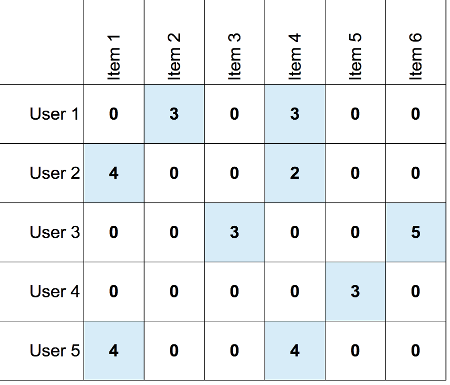
\includegraphics{sparse_matrix_sm.png}
\caption{}
\end{figure}

    \subsubsection{Colaborative filtering approach
item-item}\label{colaborative-filtering-approach-item-item}

    \begin{Verbatim}[commandchars=\\\{\}]
{\color{incolor}In [{\color{incolor}9}]:} \PY{c+c1}{\PYZsh{} Iterator for cross\PYZhy{}validation}
        \PY{n}{kf} \PY{o}{=} \PY{n}{KFold}\PY{p}{(}\PY{n}{n\PYZus{}splits}\PY{o}{=}\PY{l+m+mi}{3}\PY{p}{)}
        
        \PY{n}{sim\PYZus{}options} \PY{o}{=} \PY{p}{\PYZob{}}\PY{l+s+s1}{\PYZsq{}}\PY{l+s+s1}{name}\PY{l+s+s1}{\PYZsq{}}\PY{p}{:} \PY{l+s+s1}{\PYZsq{}}\PY{l+s+s1}{cosine}\PY{l+s+s1}{\PYZsq{}}\PY{p}{,}
                       \PY{l+s+s1}{\PYZsq{}}\PY{l+s+s1}{user\PYZus{}based}\PY{l+s+s1}{\PYZsq{}}\PY{p}{:} \PY{k+kc}{False}  \PY{c+c1}{\PYZsh{} aproach item\PYZhy{}item }
                      \PY{p}{\PYZcb{}}
                
        \PY{n}{algo} \PY{o}{=} \PY{n}{KNNBasic}\PY{p}{(}\PY{n}{sim\PYZus{}options}\PY{o}{=}\PY{n}{sim\PYZus{}options}\PY{p}{)}
        
        \PY{k}{for} \PY{n}{trainset}\PY{p}{,} \PY{n}{testset} \PY{o+ow}{in} \PY{n}{kf}\PY{o}{.}\PY{n}{split}\PY{p}{(}\PY{n}{data}\PY{p}{)}\PY{p}{:}
        
            \PY{c+c1}{\PYZsh{} Fit and run the algorithm.}
            \PY{n}{algo}\PY{o}{.}\PY{n}{fit}\PY{p}{(}\PY{n}{trainset}\PY{p}{)}
            \PY{n}{predictions} \PY{o}{=} \PY{n}{algo}\PY{o}{.}\PY{n}{test}\PY{p}{(}\PY{n}{testset}\PY{p}{)}
        
            \PY{c+c1}{\PYZsh{} Evaluate the performance calculating RMSE error}
            \PY{n}{accuracy}\PY{o}{.}\PY{n}{rmse}\PY{p}{(}\PY{n}{predictions}\PY{p}{,} \PY{n}{verbose}\PY{o}{=}\PY{k+kc}{True}\PY{p}{)}
\end{Verbatim}


    \begin{Verbatim}[commandchars=\\\{\}]
Computing the cosine similarity matrix{\ldots}
Done computing similarity matrix.
RMSE: 0.9961
Computing the cosine similarity matrix{\ldots}
Done computing similarity matrix.
RMSE: 0.9910
Computing the cosine similarity matrix{\ldots}
Done computing similarity matrix.
RMSE: 0.9911

    \end{Verbatim}

    \subsubsection{Colaborative filtering approach
user-user}\label{colaborative-filtering-approach-user-user}

    \begin{Verbatim}[commandchars=\\\{\}]
{\color{incolor}In [{\color{incolor}20}]:} \PY{c+c1}{\PYZsh{} Iterator for cross\PYZhy{}validation}
         \PY{n}{kf} \PY{o}{=} \PY{n}{KFold}\PY{p}{(}\PY{n}{n\PYZus{}splits}\PY{o}{=}\PY{l+m+mi}{3}\PY{p}{)}
         
         \PY{n}{sim\PYZus{}options} \PY{o}{=} \PY{p}{\PYZob{}}\PY{l+s+s1}{\PYZsq{}}\PY{l+s+s1}{name}\PY{l+s+s1}{\PYZsq{}}\PY{p}{:} \PY{l+s+s1}{\PYZsq{}}\PY{l+s+s1}{pearson\PYZus{}baseline}\PY{l+s+s1}{\PYZsq{}}\PY{p}{\PYZcb{}}
                 
         \PY{n}{algo} \PY{o}{=} \PY{n}{KNNBasic}\PY{p}{(}\PY{n}{sim\PYZus{}options}\PY{o}{=}\PY{n}{sim\PYZus{}options}\PY{p}{)}
         
         \PY{k}{for} \PY{n}{trainset}\PY{p}{,} \PY{n}{testset} \PY{o+ow}{in} \PY{n}{kf}\PY{o}{.}\PY{n}{split}\PY{p}{(}\PY{n}{data}\PY{p}{)}\PY{p}{:}
         
             \PY{c+c1}{\PYZsh{} Fit and run the algorithm.}
             \PY{n}{algo}\PY{o}{.}\PY{n}{fit}\PY{p}{(}\PY{n}{trainset}\PY{p}{)}
             \PY{n}{predictions} \PY{o}{=} \PY{n}{algo}\PY{o}{.}\PY{n}{test}\PY{p}{(}\PY{n}{testset}\PY{p}{)}
             
             \PY{c+c1}{\PYZsh{} Evaluate the performance calculating RMSE error}
             \PY{n}{accuracy}\PY{o}{.}\PY{n}{rmse}\PY{p}{(}\PY{n}{predictions}\PY{p}{,} \PY{n}{verbose}\PY{o}{=}\PY{k+kc}{True}\PY{p}{)}
             \PY{n}{accuracy}\PY{o}{.}\PY{n}{fcp}\PY{p}{(}\PY{n}{predictions}\PY{p}{,} \PY{n}{verbose}\PY{o}{=}\PY{k+kc}{True}\PY{p}{)}
\end{Verbatim}


    \begin{Verbatim}[commandchars=\\\{\}]
Estimating biases using als{\ldots}
Computing the pearson\_baseline similarity matrix{\ldots}
Done computing similarity matrix.
RMSE: 1.0061
FCP:  0.6477
Estimating biases using als{\ldots}
Computing the pearson\_baseline similarity matrix{\ldots}
Done computing similarity matrix.
RMSE: 1.0137
FCP:  0.6428
Estimating biases using als{\ldots}
Computing the pearson\_baseline similarity matrix{\ldots}
Done computing similarity matrix.
RMSE: 1.0242
FCP:  0.6398

    \end{Verbatim}

    \paragraph{Predict a rating with this
model}\label{predict-a-rating-with-this-model}

    \begin{Verbatim}[commandchars=\\\{\}]
{\color{incolor}In [{\color{incolor}145}]:} \PY{n}{two\PYZus{}ratings} \PY{o}{=} \PY{n+nb}{list}\PY{p}{(}\PY{n}{algo}\PY{o}{.}\PY{n}{trainset}\PY{o}{.}\PY{n}{all\PYZus{}ratings}\PY{p}{(}\PY{p}{)}\PY{p}{)}\PY{p}{[}\PY{l+m+mi}{0}\PY{p}{:}\PY{l+m+mi}{2}\PY{p}{]}
          
          \PY{n}{uid} \PY{o}{=} \PY{n}{algo}\PY{o}{.}\PY{n}{trainset}\PY{o}{.}\PY{n}{to\PYZus{}raw\PYZus{}uid}\PY{p}{(}\PY{n}{two\PYZus{}ratings}\PY{p}{[}\PY{l+m+mi}{0}\PY{p}{]}\PY{p}{[}\PY{l+m+mi}{0}\PY{p}{]}\PY{p}{)}  \PY{c+c1}{\PYZsh{}user id }
          \PY{n}{iid} \PY{o}{=} \PY{n}{algo}\PY{o}{.}\PY{n}{trainset}\PY{o}{.}\PY{n}{to\PYZus{}raw\PYZus{}iid}\PY{p}{(}\PY{n}{two\PYZus{}ratings}\PY{p}{[}\PY{l+m+mi}{1}\PY{p}{]}\PY{p}{[}\PY{l+m+mi}{1}\PY{p}{]}\PY{p}{)}  \PY{c+c1}{\PYZsh{}item id }
          
          \PY{c+c1}{\PYZsh{} rating prediction for this user and this item.}
          \PY{n}{pred} \PY{o}{=} \PY{n}{algo}\PY{o}{.}\PY{n}{predict}\PY{p}{(}\PY{n}{uid}\PY{p}{,} \PY{n}{iid}\PY{p}{,}  \PY{n}{verbose}\PY{o}{=}\PY{k+kc}{True}\PY{p}{)}
\end{Verbatim}


    \begin{Verbatim}[commandchars=\\\{\}]
user: 631        item: 1584       r\_ui = None   est = 3.79   \{u'actual\_k': 23, u'was\_impossible': False\}

    \end{Verbatim}

    \subsubsection{Kaggle}\label{kaggle}

https://www.kaggle.com/

There are a lot of available datasets and notebooks with data analysis
and recomendations.

    \subsubsection{This notebook can be
downloaded...}\label{this-notebook-can-be-downloaded...}

https://github.com/mcharnelli/PyDataCordoba2018

    \begin{figure}[htbp]
\centering

\includegraphics{questions.jpg}
\caption{}
\end{figure}

    \begin{figure}[htbp]
\centering
\includegraphics{Thankyou.gif}
\caption{}
\end{figure}

    \subsubsection{Contact}\label{contact}

https://www.linkedin.com/in/mar\%C3\%ADa-emilia-charnelli-385253160/

maria.emilia.charnelli@gmail.com


    % Add a bibliography block to the postdoc
    
    
    
    \end{document}
